% @Author: Taha Bouhsine


%%%%%%%%%%%%%%%%%%%%%%%%%%%%
% CHAPTER                  %
%%%%%%%%%%%%%%%%%%%%%%%%%%%%
\setcounter{mtc}{6}

\chapter*{Introduction}
\label{chap:general_intorduction}
\minitoc
\markboth{\MakeUppercase{Introduction}}{}%
\addcontentsline{toc}{chapter}{Introduction}%
\begin{figure}[!ht]
      \center
      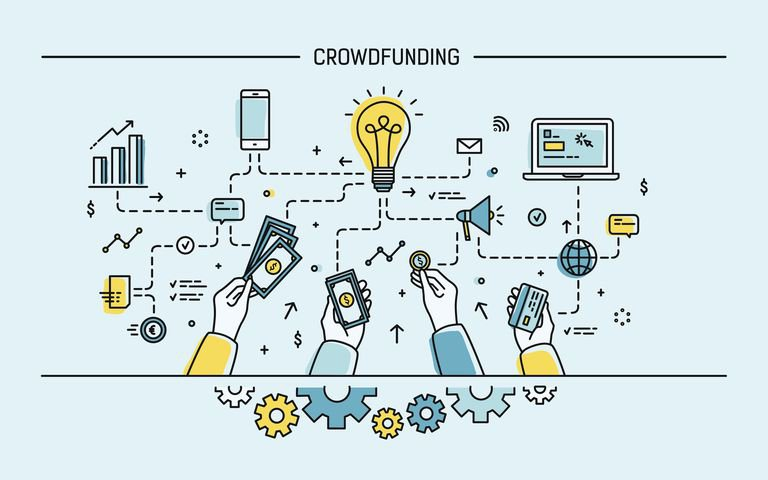
\includegraphics[scale=0.55]{assets/crowdfunding.jpg}
      \label{fig:cwdfnd}
\end{figure}

\section*{Crowdfunding}
In recent years, crowdfunding has emerged as a revolutionary financing model that allows small entrepreneurs to raise funding in the early stages of their projects, particularly those that may otherwise struggle to obtain capital (Kuppuswamy and Bayus 2013; Belleflamme et al. 2014). Today, there are approximately 1250 active crowdfunding platforms across the world, which together channeled \$16.2 billion in 2014, representing a 167 \% increase from \$6.1 billion in 2013 (Massolution 2015). Having their project successfully funded is crucial to project creators as it provides not only initial funds for project development but also access to valuable future resources, and eventually turn their projects into successful entrepreneurial organizations. Previous research shows that only 45 \% of the projects on these platforms are successfully funded. As a result, identifying general antecedents of funding success has been of great interest to researchers because it can provide insights to project creators to maximize their funding success.

Which made Crowdfunding One of the biggest topics discussed around the business community for the past few years, the idea of crowdfunding using an online platform is a great tool for building capital for a startup, funding growth for your company, or development of services or products to further your business.

New crowdfunding platforms and websites are popping up regularly to meet the needs of the expanding market, with plenty of room to benefit from the advantages of this technology by creating a crowdfunding platform.


\subsection*{Definition}
Crowdfunding is the practice of raising money from a large number of individuals for the purposes of financing a project, venture, business, or cause. Traditionally, crowdfunding has been carried out via subscriptions, benefit events, and door-to-door fundraising. However, today the term is typically associated with raising money through website platforms, which allows crowdfunding to reach a larger pool of potential funders.

% \subsection*{History}
% Crowdfunding may seem like a new idea, but in actuality, it has a long and rich history with roots going back to the 1700s.\\
% However, modern-day crowdfunding, where people and businesses raise small amounts of money from a large group of people, usually online, has its origins in 1997.

% \paragraph*{1700’s: The Irish Loan Fund}
% The Irish Loan Fund was established by author and Irish nationalist Jonathon Swift in the early 1700s as a way to provide loans to poor but creditworthy people in Dublin.

% The Fund was successful and sparked a wave of imitations, as well as an official Loan Fund Board in 1837.

% By 1843, there were approximately 300 loan funds in Ireland.

% \paragraph*{1852: The Creation of Credit Unions}
% A credit union is a non-profit bank that gets their loaning money from members, who also get part ownership and voting power in the credit union.

% In 1846, Herman Schulze-Delitzsch created a cooperatively owned bakery and mill in response to crop failure and famine in Germany.

% Six years alter, Schulze-Delitzsch and Friedrich Raiffeisen took that idea of cooperative ownership and turned it on finance, creating the first credit union.

% German credit unions had democratic governance, the member-elected board of directors, were volunteer-run, and gave each member an equal vote, regardless of how much money they contributed.

% \paragraph*{1976: The Grameen Bank and Microfinance}
% In 1976, Professor Muhammad Yunus launched a research project, where he loaned \$27 to 42 poor women in Jobra, Bangladesh.

% The project was so successful that it led to the development of the Grameen Bank Project, which is widely credited as being the first example of modern microfinance.

% Like the Irish Loan Fund, microfinance provides loans to people living in poverty who do not have access to traditional forms of credit.

% \paragraph*{1997: The Inception of Modern Day Crowdfunding}
% The first recorded successful instance of crowdfunding occurred in 1997 when a British rock band called Marillon funded their reunion tour through online donations from fans, who were eager for them to come on tour in the United States.

% Keyboardist Mark Kelly sent out an email to his 1,000 person mailing list, telling them that the band would lose about \$60k if they went on tour.

% The fans said: So why don’t we raise the money?

% One fan even volunteered to put the money in escrow in his bank account in North Carolina, to be returned if not enough was raised.

% The campaign ended up raising the money and the band went on tour. But the impact of that email resonated far beyond one music tour.

% Inspired by this innovative method of financing, ArtistShare became the first dedicated crowdfunding platform — focusing on musicians who wanted to raise money either to produce albums or go on tour — in 2001.

% Shortly thereafter, more crowdfunding platforms based on the Marillon model began to emerge, including IndieGoGo in 2007 and Kickstarter in 2009.

% \paragraph*{2006: First Use of the Term “Crowdfunding”}
% The first recorded use of the term “crowdfunding” was in August 2006, by entrepreneur Michael Sullivan.

% Sullivan used it in the launch of his company Fundavlog, which was a (failed) attempt to create an incubator for videoblog projects.

% \paragraph*{2009 – 2015 : Crowdfunding Emerges as a Major Funding Source}
% The launch of Kickstarter and IndieGoGo led to an explosion of niche crowdfunding platforms.

% The crowdfunding industry has quickly emerged as a popular option for entrepreneurs to validate their ideas, gain exposure, and gain funding.

% Crowdfunding revenue tripled from \$530 million in 2009 to \$1.5 billion in 2011.

% By 2012, there were more than 450 crowdfunding platforms, which raised more than \$2.7 billion worldwide.

% By 2015, that number had jumped to \$24.4 billion.


\subsection*{ Crowdfunding Models}
Crowdfunding facilitates the raising of capital for a variety of purposes, using numerous variations of the model. Below is a typology of how the operators in the market can potentially be segregated. The majority of platforms can be categorized under these four types, but there are several variations, such as hybrid models and those platforms that define themselves in a sectoral vertical rather than by the type of finance they provide.
\begin{enumerate}
      \item Donation Model: 
            The donation model of crowdfunding is a means for charities, or those who raise money for social or charitable projects, to gather a community online and to enable them to donate to a project. While most established charities facilitate this through their own website, crowdfunding is popular for small organizations and people raising money for personal or specific charitable causes.
      \item Lending Model: 
            Crowdfunded lending is largely an evolution of the peer–to–peer model of lending. Projects or businesses seeking debt apply through the platform uploading their pitch, with members of the crowd taking small chunks of the overall loan.
      \item Reward Model: 
            The model allows people to contribute to projects and receive non–financial rewards in return, usually operating a tiered system where the more you donate the better the reward you receive. The model often closely resembles philanthropy with the donation far exceeding the monetary value of the reward or the reward costing the fundraiser little, such as experience or recognition–related rewards.
            In these cases, entrepreneurs or artists crowdfund the production cost of their record, movie, game or product and allow the donors to be the first recipients once the production is complete. 
      \item Investment Model: 
            The final type is the application of crowdfunding to investing for equity, or profit/revenue sharing in businesses or projects. This form of the model has been the slowest to grow due to regulatory restrictions that relate to this type of activity.
\end{enumerate}


\subsection*{ How big is crowdfunding? }
In 2015, crowdfunding raised \$34 Billion worldwide and the total had doubled every year for the previous four years! Many crowdfunding campaigns are for quite small sums but some are very large. The model of crowdfunding which raised the most money is the lending model. In the UK crowdfunding in 2015 totaled £1,112 million and this figure is expected to continue to rise.


\subsection*{ Why is crowdfunding growing? }
Making a public call to fundraise from the crowd is not a new idea but crowdfunding as we now understand it has grown very quickly for several reasons since its emergence in the 1990s. These include:
\begin{enumerate}
      \item
            Technological developments : The emergence of wide and low-cost access to the internet and communication tools like social media means it is easier and cheaper for us to reach out to much more widely dispersed and larger groups of people.
      \item
            Societal changes : These technical changes have also empowered us to take on new activities that were once controlled by gatekeepers. We can see this in the way people write and publish books, publish music, writing blogs, and the general sharing of our lives online. Crowdfunding is just the financial manifestation of this sense of empowerment and the ability to take “ownership” of a process. At the same time, we are also increasingly comfortable with transacting financially online be it shopping and e-commerce or checking our bank balances. This confidence to use money online is essential for the growth of crowdfunding.
      \item
            Economic factors : The other key factor in the extraordinary growth of crowdfunding is that after the financial crisis of 2008 access to funding has been more problematic and so people are exploring alternatives to the traditional sources. At the same time interest rates have fallen to historically low levels and so “retail investors” are looking for better places to put their investments and some crowdfunding campaigns seem to offer better returns than would be available on the high street.
\end{enumerate}

\subsection*{Principe }
The other important variation in crowdfunding is the distinction between what is known as the “Keep It All” and “All Or Nothing” models.

In a “Keep It All” campaign, you keep everything you raise regardless of whether you reach your target or not.

In an “All Or Nothing” campaign you only get to keep what you raise if you succeed in reaching your target.

Crowdfunding can be undertaken by both individuals and organizations.


%%%%% 
\subsection*{ Downsides of Crowdfunding}
\begin{enumerate}
      \item It is not easy, to be a success takes a lot of time and effort to carry out the continued promotion of your campaign.
      \item Many campaigns are unsuccessful and the successful ones take work, preparation, and effort to make them happen, there is no guarantee of success but work, preparation, and effort can increase the chances of success.
      \item It is also a very public process and so you must be prepared to be open and honest in a public arena and expect brickbats and bouquets in equal measure, it is important to accept that there may be public scrutiny of your project and prepare for this.
      \item Reputation considerations: there are many aspects to this, including your appearance on the platform in the first place. Might customers and others view it negatively? There are also significant expectations from investors if your crowdfunding campaign is successful. If it meets delays or runs into problems, the reputation of your company might become damaged. Finally, by putting your idea onto a crowdfunding platform before you’re ready to bring it to the wider market (i.e. before it’s fully developed and tested), you are leaving your company open to public criticism of your plans, idea, or business.
\end{enumerate}
%%%%%%%


\subsection*{ Benefits of Crowdfunding }
\begin{enumerate}
      \item It is a very accessible process which is open to all and can be carried out on your terms
      \item you decide on the amount you want to raise and the timescale to raise the funds.
      \item You are in control, the promotion and selling of the project is the responsibility of your group.
      \item It can bring much more than money, it can attract new people and support (nonfinancial) to your group.
      \item What money it does bring can be very different from a traditional investment, funds raised through crowdfunding are unrestricted and can be used for all elements of your project.
      \item It can be quick, as you are in control you can work quickly to start raising funds.
      \item You will also produce a very valuable asset for you or your organization as you run a campaign and that “crowd asset” can be a very useful and enduring resource, people who support your project are also likely to support your group.
      \item It’s a quick and easy way to get a lot of exposure for your brand and for your new idea or initiative
      \item You can engage directly with investors who could also become your customers
      \item There is a low barrier to entry, often much lower than with other forms of investment
      \item It’s an easy way to get feedback on your idea
\end{enumerate}


% \subsection*{ What makes crowdfunding different from other funding? }
% Crowdfunding reaches widely by using technology and reduces the size of funding each individual contributor has to come up with. This means that more people can take part in.
% Making it easy for a wider group of people to support a business or project introduces a wider range of motivations for people to back a campaign. This means that there is a range of reasons why people might support you, and not simply for a financial return.
% The idea of many small contributions making a difference (as opposed to a small number of large contributions) is a concept underpinning lots of online activities that have disrupted traditional industries and it is called “The Long Tail”.
% Because the process of crowdfunding is a very public one and involves many people it can, and does, bring many more advantages than simply money. It can be a powerful campaigning tool, it can build networks, validate an idea, build awareness, and many other things, all of which can be very valuable and useful. A good crowdfunding campaign will recognize and target these additionalities.
% For some entrepreneurial projects, it has the advantage of accelerating the process of setting up a business by allowing the entrepreneur to run in parallel a series of processes like market research, publicity, marketing, and fundraising, which have often traditionally been seen as sequential.







\subsection*{ Existent Platforms }
Non-Profit:
\begin{itemize}
      \item
            Fundly: This is probably the best known of the non-profit crowdfunding sites. This platform charges a fee for all campaigns and a small transaction fee for processing. It offers a customizable donation page, with an integrated mobile experience. You can use multiple media formats to promote your cause as well as blogging.
      \item
            Salsa: This p2p platform offers branded marketing materials for every supporter and customizes messages as well. This is a fully integrated system with Salsa CRM. So, if you already use that, software data is transferred easily.
      \item
            Soapbox Engage: This is a social change platform that offers not only the ability to create cause for donation but allows you to create forms, petitions, and events to further your cause.
      % \item
      %       Bonfire: is a crowdfunding platform that allows you to create custom t-shirts to raise money for your projects. You create the t-shirt and then build a custom web page to market and use as a landing spot to drive your social media marketing campaigns.
\end{itemize}
Business:
\begin{itemize}
      \item
            Kickstarter: This is a crowdfunding platform that allows you to market potential products or businesses for investors to donate to. You create a custom page for your book, game, or any other creative project and then set a goal and start building funds. Each project will set up designated donations that have rewards attached to them.
      \item
            Indigogo: This is a great sight for startups and creatives that uses similar methods to Kickstarter. You set up a custom page and goals and market your campaign. They have integrated systems to help with the fulfillment of delivery, mobile management, perk options, etc.
      \item
            Seedrs: This crowdfunding platform uses equity investing to raise funds for small businesses and startups. It has three options to invest whether equity, funds, or convertible donations and allows other investors a discount in the future.
      
\end{itemize}




\subsection*{ Crowdfunding In Morocco }
Expected since April 2018, the examination of the so-called «collaborative financing» bill is finally starting in Morocco. In the latter case, for management companies that want to propose capital investment, it will be necessary to obtain a visa from the Moroccan Capital Market Authority . The platforms must have a minimum capital of 310,000DH and the collaborative finance companies that will manage them must have a risk prevention and reduction policy.

A few researchers in the Economic field started a study \cite{crowdMorocco}, to understand the future of crowdfunding in Morocco, they started a survey with a total of 200 participants over the internet Figure \ref{fig:survey}. Surprisingly,  The majority of respondents 96\% do not even know what the word crowdfunding means, and of 5\% left most respondents that know about crowdfunding plan to have their projects with a percentage of 62\%, while 5\% answered I do not know against 33\% do not want to have their projects. However, according to the distribution by the labor force, they found that this majority consists mainly of the unemployed and students, while more than half of the workers do not want to have their projects. For those who want to have their projects, it is mainly the lack of funding , and the lack of idea and the risk of failure that prevents them, so crowdfunding can fill this gap is becoming an alternative to financing projects or even a compliment.

Finally, they found that the majority who want to start their project and who have financing problems for a percentage of 55.5\% are interested in crowdfunding to launch or develop their projects, however, the lack of information on this system is the first cause for those who are not interested in this new mode of financing, which is normal.




% \begin{subfigure}[t!]{0.4\textwidth}
%       \centering
%       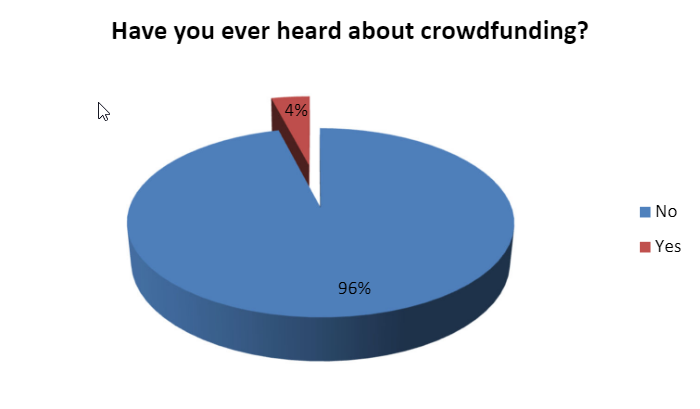
\includegraphics[width=\textwidth]{assets/heardCrowd.png}
%       \caption{ Have you heard of crowdfunding? }
%       \label{fig:heardCrowd}
%    \end{subfigure}%
%    \hfill
   
%    \begin{subfigure}[t!]{0.2\textwidth}
%          \centering
%          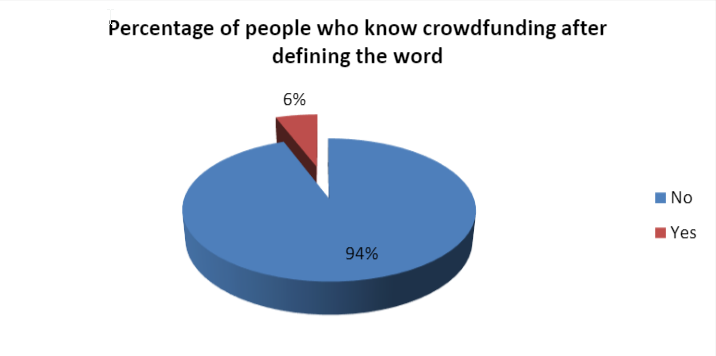
\includegraphics[width=\textwidth]{assets/knowCrowd.png}
%          \caption{After explaining the meaning of crowdfunding}
%          \label{fig:knowCrowd}
%    \end{subfigure}
%    \hfill
   
%    \begin{subfigure}[t!]{0.2\textwidth}
%          \centering
%       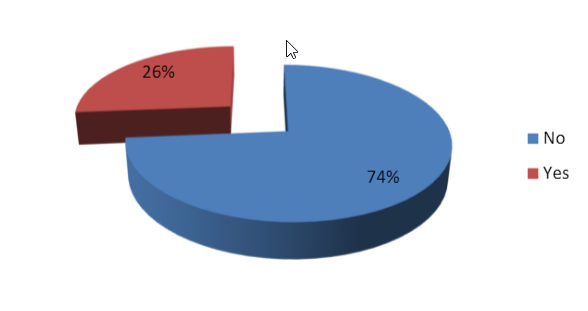
\includegraphics[width=\textwidth]{assets/knowPlatform.png}
%       \caption{Do you already know a crowdfunding platform?}
%       \label{fig:knowPlatform}
%    \end{subfigure}
%    \hfill
   
%    \begin{subfigure}[t!]{0.2\textwidth}
%          \centering
%          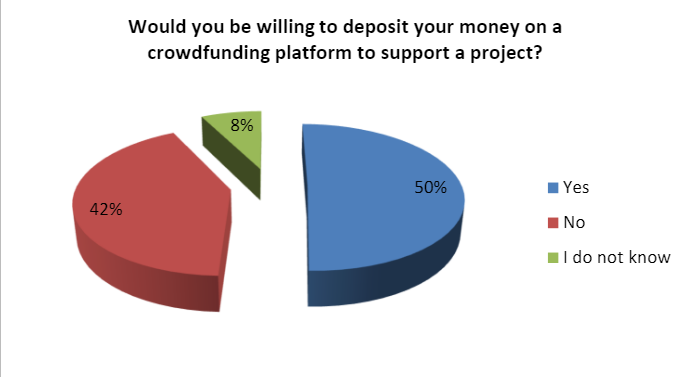
\includegraphics[width=\textwidth]{assets/willing.png}
%          \caption{Would you be to support a project on a crowdfunding platform?}
%          \label{fig:willing}
%    \end{subfigure}


      
\begin{figure}
      \centering
      \begin{subfigure}[b]{0.45\textwidth}
          \centering
          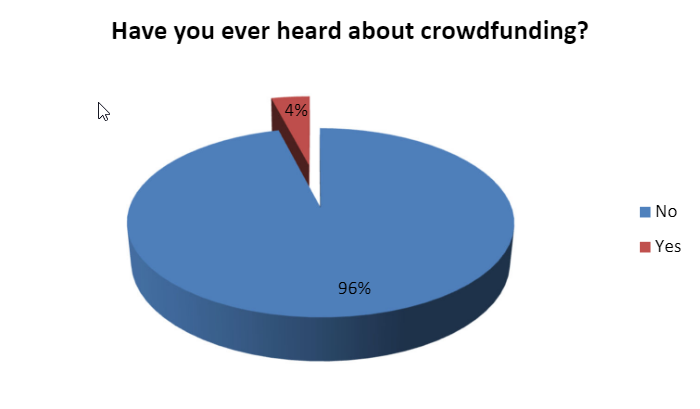
\includegraphics[width=\textwidth]{assets/heardCrowd.png}
          \caption{Have you heard of crowdfunding?}
          \label{fig: heardCrowd}
      \end{subfigure}
      \hfill
      \begin{subfigure}[b]{0.45\textwidth}
          \centering
          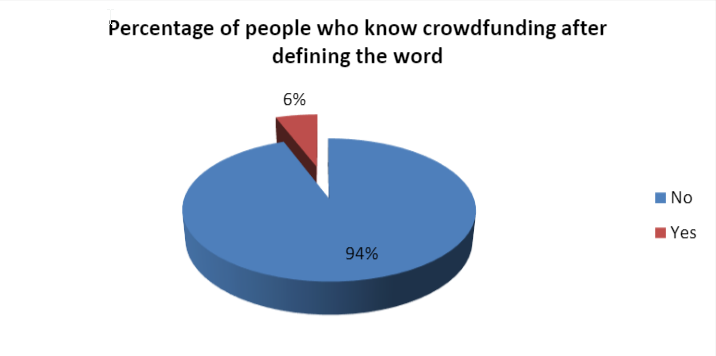
\includegraphics[width=\textwidth]{assets/knowCrowd.png}
          \caption{After explaining the meaning of crowdfunding}
          \label{fig:knowCrowd}
      \end{subfigure}
      \hfill
      \begin{subfigure}[b]{0.45\textwidth}
          \centering
          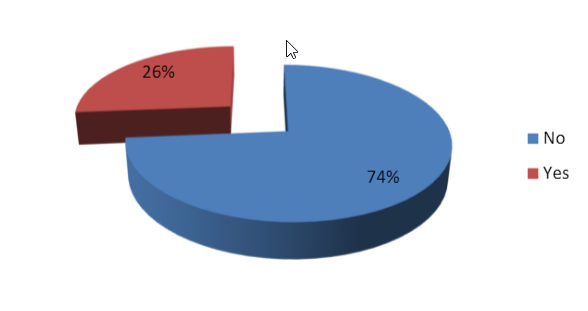
\includegraphics[width=\textwidth]{assets/knowPlatform.png}
          \caption{Do you already know a crowdfunding platform?}
          \label{fig:knowPlatform}
      \end{subfigure}
      \hfill
      \begin{subfigure}[b]{0.45\textwidth}
          \centering
          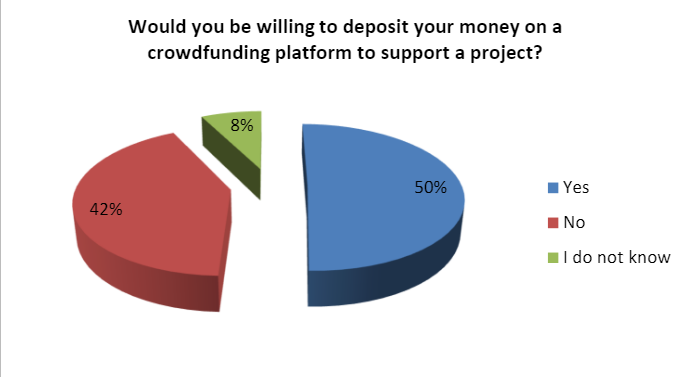
\includegraphics[width=\textwidth]{assets/willing.png}
          \caption{Would you be to support a project on a crowdfunding platform?}
          \label{fig:willing}
      \end{subfigure}
      
      \caption{Survey on crowdfunding in Morocco}
      \label{fig:survey}
\end{figure}





% \section*{ Main Actors }
% Different players are involved in crowdfunding models. First, many people propose ideas and
% projects to be funded. They want to use crowdfunding as a tool to gather financial support from interested supporters.
% Then there is the crowd of people that provides this financial support to these projects, bearing an investment
% risk and expecting a certain payoff. And finally, there is the crowdfunding platform, the intermediary that acts
% as a matchmaker between those who want to deliver the new initiatives using crowdfunding mechanisms
% and those who want to support such initiatives through their investment efforts \cite{10.1108/09564231111155079}.

% \begin{enumerate}
%       \item Creator:
%             Or capital seekers, are mainly concerned with their motivations to get involved in crowdfunding, the determinants of success, and the legal restrictions of equity-based crowdfunding \cite{10.1007/978-3-319-18017-5_3}.

%       \item Funder:
%       Or capital providers, are essential to the success of a crowdfunding campaign. Interesting research can be performed on the motives of this unique group of investors for participating in crowdfunding. One thing that
%             makes this group so special is that they are not exclusively motivated by earning money.

% \end{enumerate}